%----------------------------------------------------------------------------
%bb defines the bounding box for the pdf
%viewport defines the area of the pdf used
%in sidewaysfigure the last entry in bb moves the caption toward/away the pic
%in sidewaysfigure the second entry in bb moves the pic toward/away the caption
%----------------------------------------------------------------------------
\begin{figure}
\scalebox{0.6}[0.6]{
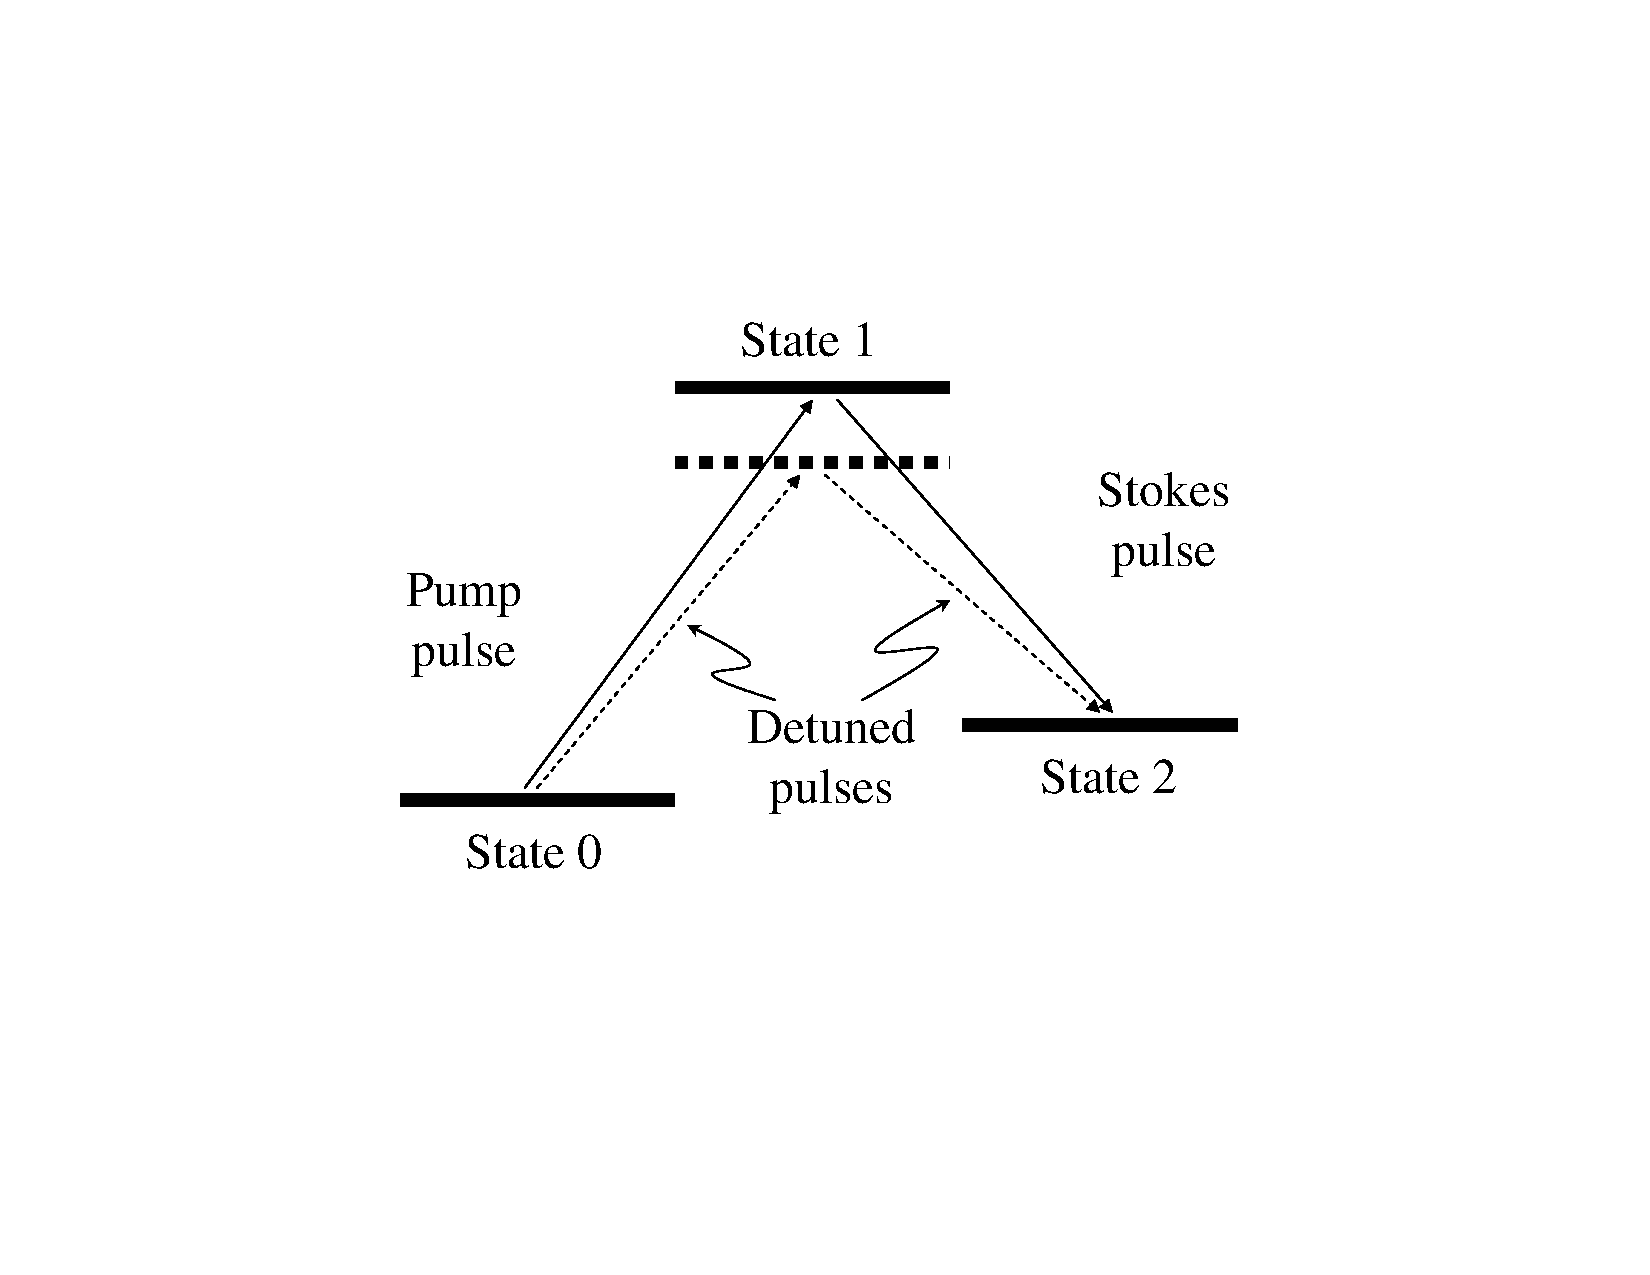
\includegraphics[bb=35 180 489 450]
{sp_detuning/sp_detuning.pdf}
}
\caption[Stokes and pump pulses in a $\Lambda$ system]{Stokes and pump pulses in a $\Lambda$ system. Here we show the pump pulse (connecting states $\ket{0}$ and $\ket{1})$ and the stokes pulse (connecting states $\ket{1}$ and $\ket{2})$. In Figure \ref{amp_surface} we show the effect of amplitude variations on the residue. Also shown here are two \emph{equally} detuned pulses. The figure suggests that significant population will still transfer, but only when the detunings are nearly equal. See Figure \ref{ridge} for an actual calculation.}
\label{sp_detuning}
\end{figure}
%----------------------------------------------------------------------------
